% !mode::"TeX:UTF-8"
\documentclass[titlepage]{article}
%\documentclass[,twoside,doctor]{article}

\usepackage{graphicx}
%\usepackage{pdfpages}
\graphicspath{{image/}{sch/}}
%\graphicspath{}

\usepackage{amsmath}
\usepackage{amssymb}
\usepackage{ctex}
\usepackage{geometry}
\geometry{left=2.5cm,right=2.5cm,top=3cm,bottom=3cm}
\usepackage{fancyhdr}
\pagestyle{fancy}
\fancyfoot{} % clear all footer fields
\fancyfoot[L]{RT-Thread 启动下一代实时操作系统演化}
\fancyfoot[R]{\thepage}
\renewcommand{\footrulewidth}{0.5pt}
%\usepackage{pdfpages}
%\usepackage{epsfig}
\usepackage[colorlinks,
            linkcolor=black,
            anchorcolor=blue,
            citecolor=green
            ]{hyperref}


\author{RT-Thread工作室}
\title{RealTouch用户手册}

\begin{document}
\maketitle
 \renewcommand{\contentsname}{目录}
 \tableofcontents
 \newpage
 \section{简介}
RealTouch是RT-Thread OS的一个评估演示板,板子使用意法半导体公司的Cotex-M4内核的STM32F407ZGT6为核心,几乎完全使用了F4的外设,
包括以太网,I2S,FSMC。。。外扩的CAN,RS232方便同其他外设通讯,预留的SWD接口更能方便的连接仿真器调试程序,支持的SDIO接口的SD卡,
方便评估RT-Thread的文件系统,显示部分一个7寸的800*480LCD方便评估RT-Thread的GUI。
\newpage
\section{RealTouch演示板}
\begin{figure}[h]
 \centering
 \includegraphics[width=0.7\textwidth]{board_d.jpg}
 \caption{RealTouch演示板}
 \end{figure}
\newpage
\section{概述}
\subsection{特性}
 \begin{itemize}
 \item 支持两个DC电源输入
    \begin{itemize}
    \item[-] 一个标准DC电源插座(Φ3.5mm)
    \item[-] 一个mini USB A接口
    \end{itemize}
 \item 7寸800*480的LCD面板
 \item 4线电阻触摸屏
 \item 一路RS232
 \item IEEE802.3-2002以太网接口
 \item IEEE802.11 b/g/n wifi接口
 \item I2S DAC,立体声音频输入、输出接口
 \item 一个CAN2.0接口
 \item 标准4线SD卡接口(使用SDIO)
 \item 16Mbit串行Flash
 \item 512Kbitx16 SRAM
 \item 2Gbit NAND Flash(K9F2G08U0B)
 \item 一个双向红外通讯接口
 \item USB OTG全速接口
 \item USB Bus ESD保护
 \item SWD调试接口(接口兼容20pin ARM JTAG接口)
 \item RTC
 \end{itemize}

  \subsection{软件支持}
  \subsubsection{关注 RealTouch}
 作为一个RT-Thread的评估板,所有例程皆是在RT-Thread下运行的,RT-Thread RTOS是一款来自中国的开源实时操作系统,
 由国内一些专业开发人员开发、维护。它不仅仅是一款高效、稳定的实时核心,也是一套面向嵌入式系统的软件平台,覆盖了全抢占的实时操作系统内核,
 小巧而与底层具体实现无关的文件系统,轻型的TCP/IP协议栈以及轻型的多窗口多线程图形用户界面。RT-Thread实时操作系统0.3.x/1.0.x系列版本遵循GPLv2许可证。

 相关信息请关注:www.rt-thread.org/realtouch
 \subsubsection{取得RealTouch代码}
 RealTouch是一个开源软硬件评估板,使用分布式版本控制/软件配置管理软件GIT来管理代码,并托管在GitHub,RealTouch在GitHub上的地址是:https://github.com/RT-Thread/realtouch-stm32f4
\newpage
\section{PCB布局}

 \begin{figure}[h]
 \centering
 \includegraphics[width=0.65\textwidth]{board_info.eps}
 \caption{PCB布局}
 \end{figure}
\newpage
\section{硬件方框图}

 \begin{figure}[h]
 \centering
 \includegraphics[width=16cm]{bus.png}
 \caption{框图}
 \end{figure}
 \newpage
 \section{硬件描述}
 \subsection{电源}
 \begin{figure}[h]
 \centering
 \includegraphics[width=15cm]{power.png}
 \caption{电源}
 \end{figure}
RealTouch输入电源电压为DC5V,800mA。请确保输入电压不得超过5V,否则可能会主板。同时也可以使用USB供电,因USB输出电流有限,所以当使用USB供电时只能做不需要开启LCD背光和音频输出的实验,不然有可能引起USB电流过载。

RealTouch 电源输入部分使用一个低压差线性稳压器
AMS1117,输入连接到来自外部电源和USB的+5V,提供一个稳定的3.3V主电源。
 \subsection{LCD偏压、背光}
  \begin{figure}[h]
  \centering
  \includegraphics[width=15cm]{lcd_power.png}
  \caption{LCD电源}
 \end{figure}
 一片TPS61040和其外围电路组成的LCD偏压驱动,一片CAT4139升压芯片提供LCD的背光驱动,其接受由显示控制电路RA8875输出的PWM信号调整背光亮度。
 \newpage
 \subsection{串行Flash}
  \begin{figure}[h]
  \centering
  \includegraphics[width=15cm]{spiflash.png}
  \caption{SPI Flash}
 \end{figure}
 W25Q64是一个64Mbit的串行Flash存储器,通过SPI总线挂接在MCU上,其掉电不丢失的特性使存储一些不常更改的数据和一些常量(如触控面板的校准数据)成为可能。
 \newpage
 \subsection{时钟}
  \begin{figure}[h]
  \centering
  \includegraphics[width=11cm]{clock.png}
  \caption{时钟}
 \end{figure}
 一个25M无源晶体振荡器,提供给MCU一个稳定的25M时钟源,一个32.768K的无源晶体振荡器,和MCU的内部RTC相连,提供一个精准的RTC时钟源,由MCU的MCO(PA8)输出的HSE无分频的25M时钟,
 经过SN74LVC1G17单路斯密特触发缓冲器整形,分别提供3 路时钟信号:音频,以太网和显示控制器。
 \newpage
 \subsection{音频}
  \begin{figure}[h]
  \centering
  \includegraphics[width=15cm]{audio.png}
  \caption{音频}
 \end{figure}
 I2S立体声解码芯片WM8978和其外围电路组成了一个可录放音的I2S电路。P1,P2,两个咪头提供了立体声录音;跳线J1可与选择WM8978的MCLK来源,默认使用SN74LVC1G17整形后的25M时钟;跳线J2和MCU部分的J4,
 提供了耳机插入检测信号,可以选择由MCU还是WM8978来检测耳机的插入,默认J4是一个0R的电阻,由MCU来检测耳机插入信号,SPK是一个内置喇叭。
 \subsection{触控面板}
  \begin{figure}[h]
  \centering
  \includegraphics[width=15cm]{touch.png}
  \caption{触控面板}
 \end{figure}
 四线电阻触摸屏的X、Y连接在FPC连接座上,由专用芯片XPT2046采集面板动作,以触发MCU中断,MCU通过SPI总线来读取数据,确认动作。
 \newpage
 \subsection{SRAM、NAND Flash}
  \begin{figure}[h]
  \centering
  \includegraphics[width=15cm]{sram.png}
  \caption{SRAM}
 \end{figure}
 挂接在FSMC上的512bit*16的SRAM和1G的NAND Flash,扩展了板子的存储。
 \newpage
 \subsection{SD卡}
  \begin{figure}[h]
  \centering
  \includegraphics[width=15cm]{sd.png}
  \caption{SD Card}
 \end{figure}
 RT-Thread自带的小巧,与底层硬件无关的文件系统轻松支持SDIO 4bit模式的SD卡。
 \newpage
  \subsection{键盘}
  \begin{figure}[h]
  \centering
  \includegraphics[width=15cm]{key.png}
  \caption{按键}
 \end{figure}
 RealTouch支持7个用户按键和一个启动模式选择按键(与Enter、WakeUp,S8共用),按键均直接连接到MCU的GPIO上,按键全部使用高电平有效的方式,在原理图安排中,所有按键均按照中断线一字排开,方便软件处理。
 \newpage
  \subsection{以太网}
  \begin{figure}[h]
  \centering
  \includegraphics[width=15cm]{eth.png}
  \caption{以太网}
 \end{figure}
 RealTouch拥有一个支持IEEE802.3-2002,10/100M以太网接口,使用一片LAN8720A挂接在F4的RMII接口。一个网络变压器,起到隔离和保护的作用,和一个标准的RJ45接头。
  \subsection{WiFI}
  \begin{figure}[h]
  \centering
  \includegraphics[width=15cm]{wifi.png}
  \caption{WIFI}
 \end{figure}
 RealTouch拥有一个支持IEEE802.11 b/g/n的WIFI模块。该模块是一个选配件。
 \newpage
   \subsection{LCD}
  \begin{figure}[h]
  \centering
  \includegraphics[width=15cm]{lcd.png}
  \caption{LCD}
 \end{figure}
 RealTouch使用一片LCD控制器RA8875来驱动一个7寸 800*480分辨率的TFT LCD,挂接在MCU的FSMC总线上。RA8875是一个通用的彩色LCD驱动器,内置触控面板(未使用),
 键盘扫描(未使用),以及2D图形加速等功能。更多信息请参阅RA8875数据手册。
 \newpage
  \subsection{USB OTG FS}
  \begin{figure}[h]
  \centering
  \includegraphics[width=15cm]{usb.png}
  \caption{USB}
 \end{figure}
 RealTouch支持一个标准的全速OTG接口,默认接口类型是USB-MiniA/B,PCB板预留USB-A型母座,与miniA/B不同的是,A型母座少了一根ID线。AIC1526受MCU控制,
 当外部一个设备插入,AIC1526可以提供一个标准的5V 500ma的电源供给。USBLC6-4是一个ESD保护芯片,以保护RealTouch的USB口不受损伤。
 \newpage
\section{原理图}
\subsection{RealTouch框图}
 %\includegraphics[width=16cm,angle=90]{top.eps}
  \begin{figure}[h]
  \centering
  \includegraphics[width=11cm]{top.pdf}
  \caption{top}
 \end{figure}

 \newpage
 \subsection{MCU}
  \begin{figure}[h]
  \centering
 \includegraphics[width=11cm]{cpu.pdf}
  \caption{mcu}
 \end{figure}

 \newpage
  \subsection{音频}
  \begin{figure}[h]
  \centering
 \includegraphics[width=11cm]{audio.pdf}
 \caption{audio}
 \end{figure}

 \newpage
 \subsection{电源}
 \begin{figure}[h]
  \centering
 \includegraphics[width=11cm]{power.pdf}
  \caption{power}
 \end{figure}

 \newpage
 \subsection{内存}
 \begin{figure}[h]
  \centering
 \includegraphics[width=11cm]{sram.pdf}
 \caption{sram}
 \end{figure}

 \newpage
 \subsection{显示}
 \begin{figure}[h]
  \centering
 \includegraphics[width=11cm]{lcd.pdf}
 \caption{lcd}
 \end{figure}

 \newpage
 \subsection{串行Flash}
 \begin{figure}[h]
  \centering
 \includegraphics[width=11cm]{spiflash.pdf}
 \caption{spiflash}
 \end{figure}

 \newpage
 \subsection{SD卡}
 \begin{figure}[h]
  \centering
 \includegraphics[width=11cm]{sd.pdf}
 \caption{lcd}
 \end{figure}

 \newpage
 \subsection{USB}
 \begin{figure}[h]
  \centering
 \includegraphics[width=11cm]{usb.pdf}
 \caption{usb}
 \end{figure}

  \newpage
 \subsection{以太网}
 \begin{figure}[ht]
  \centering
 \includegraphics[width=11cm]{eth.pdf}
 \caption{eth}
 \end{figure}

 \newpage
 \subsection{WIFI}
 \begin{figure}[ht]
  \centering
 \includegraphics[width=11cm]{wifi.pdf}
 \caption{wifi}
 \end{figure}

 \newpage
 \subsection{键盘}
  \begin{figure}[ht]
  \centering
 \includegraphics[width=11cm]{key.pdf}
 \caption{key}
 \end{figure}



 \newpage
 \section{修订历史}

  \begin{table}[h]
  \centering
  \begin{tabular}{|l|l|l|}
  \hline
  日期 & 版本 &  内容\\
  \hline
  2012-7-25 & 2 & 更新部分图片,更新原理图\\
  \hline
  2012-5-28 & 1 &  初始版本\\
  \hline
  \end{tabular}
  \end{table}


\end{document}
